\section{Задание 5. Поток векторного поля}

\textbf{Условие.}

\begin{multicols}{2}
    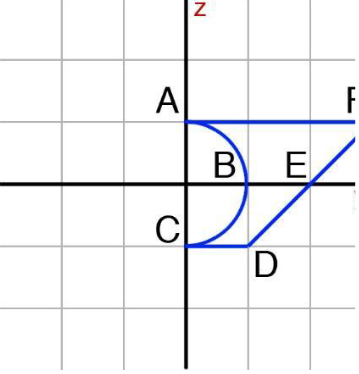
\includegraphics[height=7cm]{images/5a1}

    Дано тело $T$, ограниченное следующими поверхностями: $\displaystyle y - \sqrt{1 - x^2 - z^2} = 0, x^2 + z^2 = 1, y - z = 2$.

    На рисунке представлено сечение тела $T$ координатной плоскостью $Oyz$.

    1) Изобразите тело $T$ на графике в пространстве.

    2) Вычислите поток поля

    $\displaystyle \overrightarrow{a} = (\cos^2(z + y))\overrightarrow{i} + 2x\overrightarrow{j} + \left(\sqrt{y + 5} + 2z\right) \overrightarrow{k}$

    через боковую поверхность тела $T$, образованную вращением дуги $ABC$ вокруг оси Oy, в направлении внешней нормали поверхности тела $T$.
\end{multicols}


\vspace{10mm}
\textbf{Решение.}

It is empty but you can fill it!

\textit{Ответ}:  It is empty but you can fill it!
\clearpage
